  \chapter{Theoretical/Computational work}
  
\section{Modified Newtonian Dynamics (MOND)}

MOND is an algorithm that allows us to calculate the distribution of the effective gravitational force in astronomical objects from the distribution of baryonic matter by introducing one additional fundamental parameter that has the dimensions of acceleration. This  is done by the determining the rotation curves of disk and spiral galaxies and relating it with normal keplerian motion. \cite{dm_2}.

 It is a numeric way of calculating  the missing factor (acceleration parameter) that is causing the discrepancy in the rotation curves. It relates MOND acceleration `$a$' to Newtonian acceleration $a_{N}$ using the following formula \begin{equation}
 a_{N}= a\,\mu(\frac{a}{a_{0}})
\end{equation}
where $a_{0} = 1.2 \times 10^{-8} cm s^{-2}$  is a constant of physics.
The interpolation function $\mu (a/a_0)$ shows asymptotic behaviour $\mu=1$ when $a>> a_0$,  which reduces to the Newtonian expression in the strong field regime. For $a << a0$  these assumptions give us the following expression
\begin{equation}
a= \sqrt{a_{N}a_{0}}= \frac{\sqrt{GMa_{0}}}{r}
\end{equation}
Different functions can be used for $\mu$. Currently the most used function is
\begin{equation}
\mu (\frac{a}{a_{0}}) = \frac{\displaystyle \frac{a}{a_{0}}}{\sqrt{1+(\displaystyle \frac{a}{a_{0}})^2}}
\end{equation}
It works well for galactic rotation and solving for a, it gives
\begin{equation}
a= a_{N}(\frac{1}{2}+\frac{1}{2\sqrt{1+(\displaystyle \frac{2a_{0}}{a_{N}})^2}})^\frac{1}{2}
\end{equation}
The above expression allows us to calculate the MOND acceleration provided Newtonian gravity is known.

\section{Area of Study}
  MOND has been tested successfully on spiral galaxies, so for this research we chose the nearest spiral galaxy i.e. Andromeda Galaxy. 

\subsection{Andromeda Galaxy}
  Andromeda, M31 or NGC 224, is the nearest spiral galaxy to the Milky Way, located 744 kpc away. It is far enough to give us a convenient global view, while close enough that we can take spectra of individual stars. Its disk is highly inclined, enabling us to view the inner parts of the spheroid by studying the regions near the minor axis. 

\subsection{Distance to the Galaxy}

The stars and galaxies are at a considerable distance from Earth, from a few parsecs to several kilo and even mega parsecs. It is essential to calculate the distances in order to determine further properties of these objects. There are different techniques for calculating distances that astronomers have developed.
A few of them are listed below:

\subsubsection*{Standard Candles}
 Cepheid variable stars are used as cosmic distance ladders to measure distances. Cepheid variable stars are a part of the star cycle formed when a giant red star is about to die. These stars expand and contract, changing their brightness from brighter to dimmer \cite{stanc}.  They change their brightness in regular intervals of 1 to 70 days and the relation between the time interval and apparent magnitude gives us distances via the following equation:
 \begin{equation}
 d= 10^{\displaystyle \frac{(m-M+5)}{5}}
 \end{equation}
where \textbf{m} is the apparent magnitude and \textbf{M} is the absolute magnitude.

\subsubsection*{Binary Stars }

A binary star system consists of two stars  gravitationally bound to each other orbitting around their common centre of mass. Almost \textbf{85} percent of stars are part of a binary star system \cite{bin}. The orbital periods and relative distances of these systems vary enormously. If the stars have the same masses they are equally distant from the CM, otherwise the more massive star is closer to the CM.

Binary stars are difficult to observe directly because the systems are too distant to resolve each star. Astronomers use their light curve, how apparent brightness changes with time, to calculate the distances. Binary stars are classified into the following categories.

\begin{enumerate}

\item\textbf{Visual Binaries}

Some binary systems are close to the Earth and have a significantly large distance between eachother so they can be observed individually in a telescope \cite{sys_1}.

\item \textbf{ Spectroscopic Binaries }

Most binary systems are too far to be resolved by telescopes so they are detected by the Doppler shifts in their spectral lines. The two stars appear to be moving alternatively towards and away from us so the one moving towards us is blue shifted while the one moving away is red shifted.


\item \textbf{Astrometric Binaries}

The Binary stars sometimes are too far or too close to eachother making it hard to distinguish between the them in the system \cite{astrometric_binaries}.


\item \textbf{Eclipsing Binaries}

This type of binary system consists of two luminous stars that appear as a single point of light but due to brightness variation and spectroscopic observations we conclude that they are two stars in close orbit around each other causing them to eclipse each other \cite{eclipsing_binaries}.


These binary systems give the best estimates of distances. This system of binary stars have two luminous stars. The graph of brightness versus time is known as the light-curve of eclipsing binaries.

\begin{figure} [h]
\centering
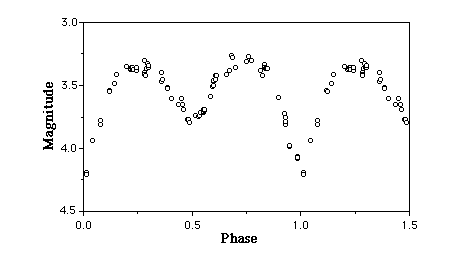
\includegraphics[scale=0.5]{LC}
\caption{Photometry of Beta Lyrae in 1992-1993 \cite{eclipsing_binaries}}
\end{figure}

\end{enumerate}

\subsubsection*{Explanation of Light Curve}

 The eclipsing movement of the stars in different phases gives the light-curve. The binary system works in the manner explained in the figure $2.2$ 
\cite{sys}
\begin{figure} [h]
\centering
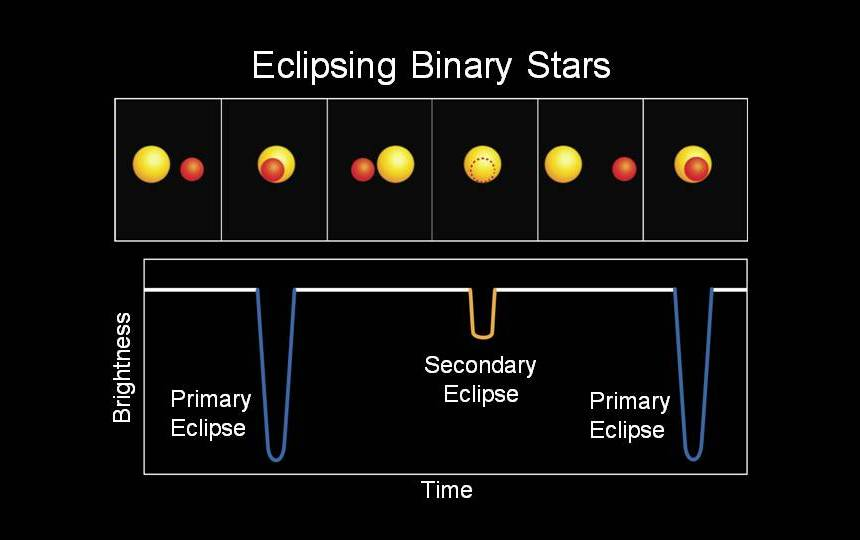
\includegraphics[scale=0.5]{Light}
\caption{Eclipsing Binary System}
\end{figure}

\section{Computational Work}
The verification of Modified Newtonian Dynamics depends upon the rotation curve of the specific galaxy. The rotation curve gives us a relation between the rotational velocity and the distance of the astronomical object from the centre of the galaxy. I chose to study the Andromeda Galaxy, our nearest neighbour. To calculate the rotation curve one needs to calculate the distances of the visible astronomical objects that comprise the galaxy and its mass distribution. Keeping the constraints of unavailability of any telescope in mind I had to work with an existing image of the Andromeda Galaxy and used the technique of Image Analysis.

\subsection{Image Analysis of M31}

Image analysis allows us to extract meaningful information from a digital image. I chose the Python language for this purpose. Python is a precise coding language that allows us to write complex code in fewer lines.

Figure \ref{andromedaimage} is an image of one quadrant of the Andromeda Galaxy released by Hubble Telescope Images in $2015$ which was used for our analysis. It is an 8-bit RGB JPEG image of width 6000 pixel and height 1918 pixels.
    
\begin{figure}[h!]
   \centering
   \includegraphics[scale=0.125]{andromeda.jpg}
   \caption{Andromeda Galaxy, M31, NGC 224}
   \label{andromedaimage}
\end{figure}

We assume that each pixel in the image corresponds to a Main Sequence star whose luminosity is related to its mass by the relation 

\begin{equation}
\frac{L}{L_{\odot}} = (\frac{M}{M_{\odot}})^4 
\end{equation}

where $L_{\odot}$ is solar luminosity and $M_{\odot}$ is solar mass \cite{LMratio}.

We further assumed the Andromeda Galaxy to be roughly circular with a cylindrically symmetric mass distribution. This allowed us to model the Andromeda Galaxy as a collection of concentric rings. 

Our task was then to analyze the image and calculate the mass of these concentric rings. We chose to divide the galaxy into $400$ concentric rings. This was achieved using the following python code.

\subsection{Program for Image Analysis}
The program was divided into different modules to create a clear concept of purpose of each module. Following are the modules of the program.
\begin{enumerate}
\item \textbf{Defining the Image Dimensions}

The following code gives us the dimensions of the image being used and the spectral type of the image as the third entity.

\begin{verbatim}
andro = misc.imread('andromeda.jpg')
(w, h,d) = andro.shape
\end{verbatim}

Output: (1918,6000,3)


\item \textbf{Calculation of the Distance of a certain pixel from the centre of the Galaxy}

This part defines the co-ordinates of the Origin as $x_{0}$ and $y_{0}$. The function iterates over the whole image to calculate the distance of each pixel from the centre of the galaxy using Pythagoras' theorem.

\begin{verbatim}
x0 = 88.23
y0 =1675.78

def calc_distance(x0,y0,x,y):

    x_dist = (x - x0)
    y_dist = (y-y0)

    return  math.sqrt(x_dist*x_dist+y_dist*y_dist)
\end{verbatim}

\item \textbf{Intensity calculation for each pixel}

The intensity of each pixel is required to estimate the mass of each astronomical object in the galaxy, as intensity is directly proportional to the energy of the celestial object [1234]. To calculate the intensity of each pixel I had to first convert it into grayscale. This was done by fetching the RGB values of each pixel and taking the square root of their squares divided by $3$. The grayscale pixel values are then normalized to fall within the range $0$ to $1$. 
\begin{verbatim}
denom = math.sqrt(3)*255

def calc_gs_intensity(i):

    R = float(i[0])
    G = float(i[1])
    B = float(i[2])

    return math.sqrt(R*R+G*G+B*B)/denom
\end{verbatim}

\item \textbf{Storing the Data}

To avoid repeating this calculation the intensity and distance data calculated was stored in an interim data file (CSV).

\begin{verbatim}
with open('data.csv', 'w') as fout:

        for x in range(w):
            for y in range(h):

                r = calc_distance(x0,y0,x,y)
                i = calc_gs_intensity( andro[x,y] )

                fout.write(str(r) + "," + str(i)+ "\n")
\end{verbatim}

\item \textbf{Histogram}

Now to analyze the mass distribution of M31 I plotted a histogram of radius versus cummulative normalized intensity. By using 400 bins to collect the data I was able to calculate the cummulative intensity in 400 concentric rings about the galactic center.

\begin{verbatim}
import matplotlib.pyplot as plt

def main():

    reader = csv.reader (open('data.csv', 'rb'), delimiter=',')

    R = []
    I = []

    for row in reader:
        r= float(row[0])
        R.append( r )
        I.append( float(row[1]) )

    plt.hist(R, weights=I, bins = 400)
    plt.xlabel('radius   (pixels)    1kpc = 11.7px  ')
    plt.ylabel('Cummulative Normalized Intensity')
    plt.show()

\end{verbatim}

\begin{figure}[ht]
   \centering
   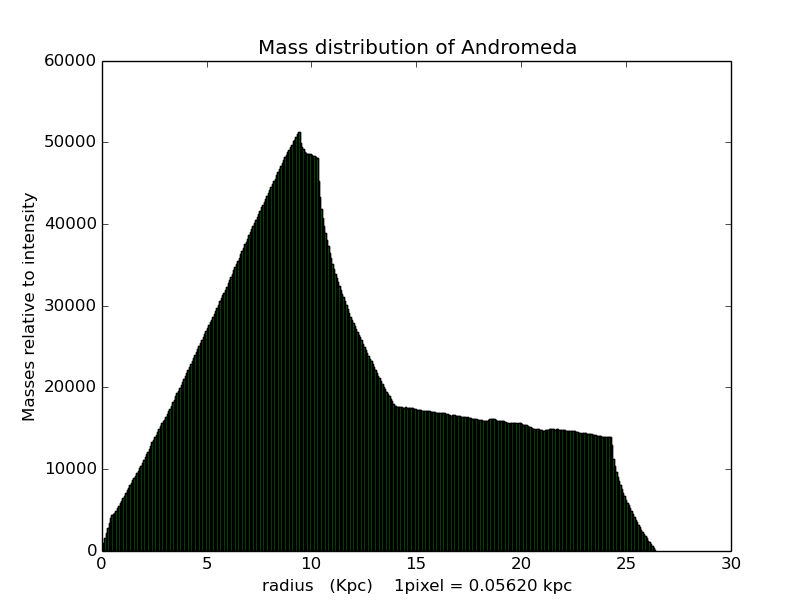
\includegraphics[scale=0.45]{400}
   \caption{Mass Distribution of the Andromeda Galaxy}
   \label{histogram}
\end{figure}

\end{enumerate}

\section{Calculation of Force}

According to Newton's second law force is directly proportional to acceleration keeping mass constant. For the calculation of force on the objects inside the galaxy we consider it to be a set of concentric rings. The histogram (Figure \ref{histogram}) gives us the mass distribution of the galaxy as a function of radius. The force on a particle at radius $r$ will be the cumulative effect of force due all of the concentric rings.

Let us consider the problem of finding the gravitational potential in all space produced by a ring of mass M. In most analytical approaches to this problem the solution is found only along the symmetry axis of the ring where the integrals evaluate to elementary functions. To solve for the force exerted by a massive ring with in the galactic plane we are required to calculate the off-axis solution that involves special functions, in this case Elliptic Integrals \cite{paper}.
 
The system I am working on is given by Figure \ref{ring}. A ring of mass M and radius R lies in the x-y plane with its centre at the origin. A mass $m$ is at a distance $r$ as described in Figure \ref{ring}, 

\centering
\begin{minipage}[b]{0.4\textwidth}
      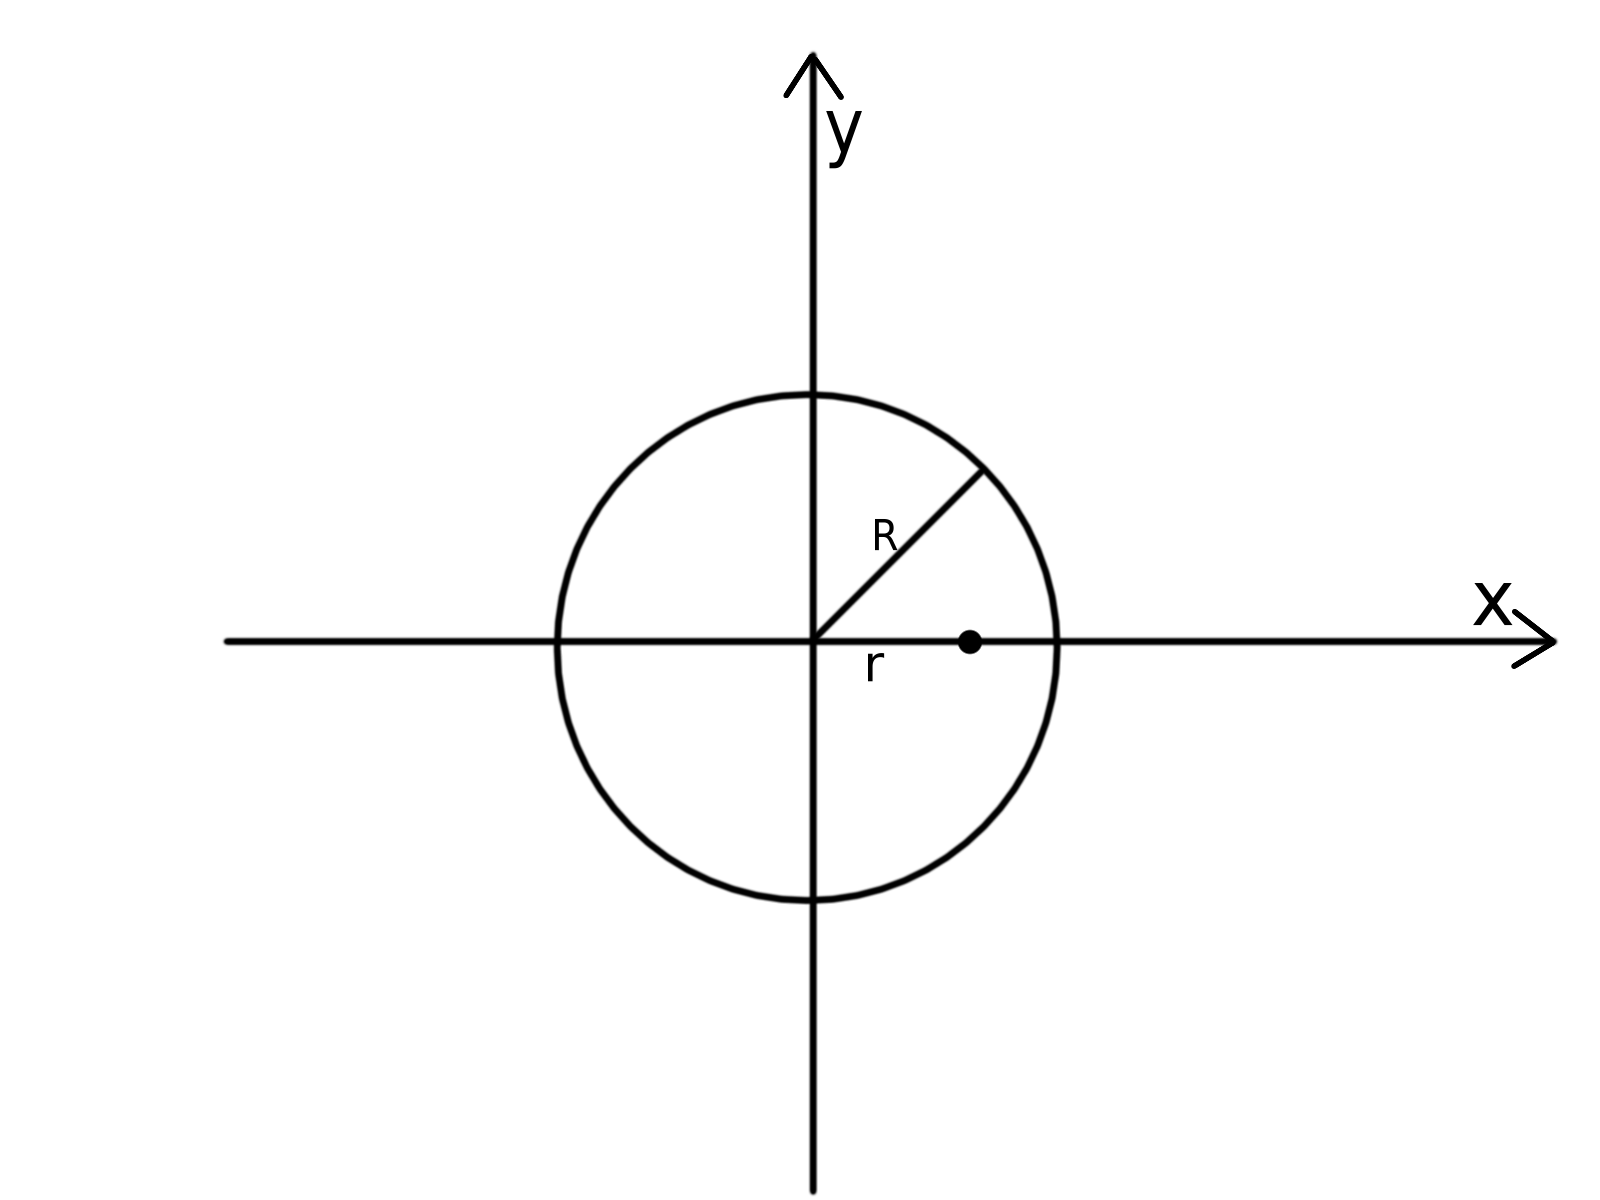
\includegraphics[width=\textwidth]{fig2}
      \captionof{figure}{Ring of Mass}
      \label{ring}
\end{minipage}
\hfill
\begin{minipage}[b]{0.4\textwidth}
      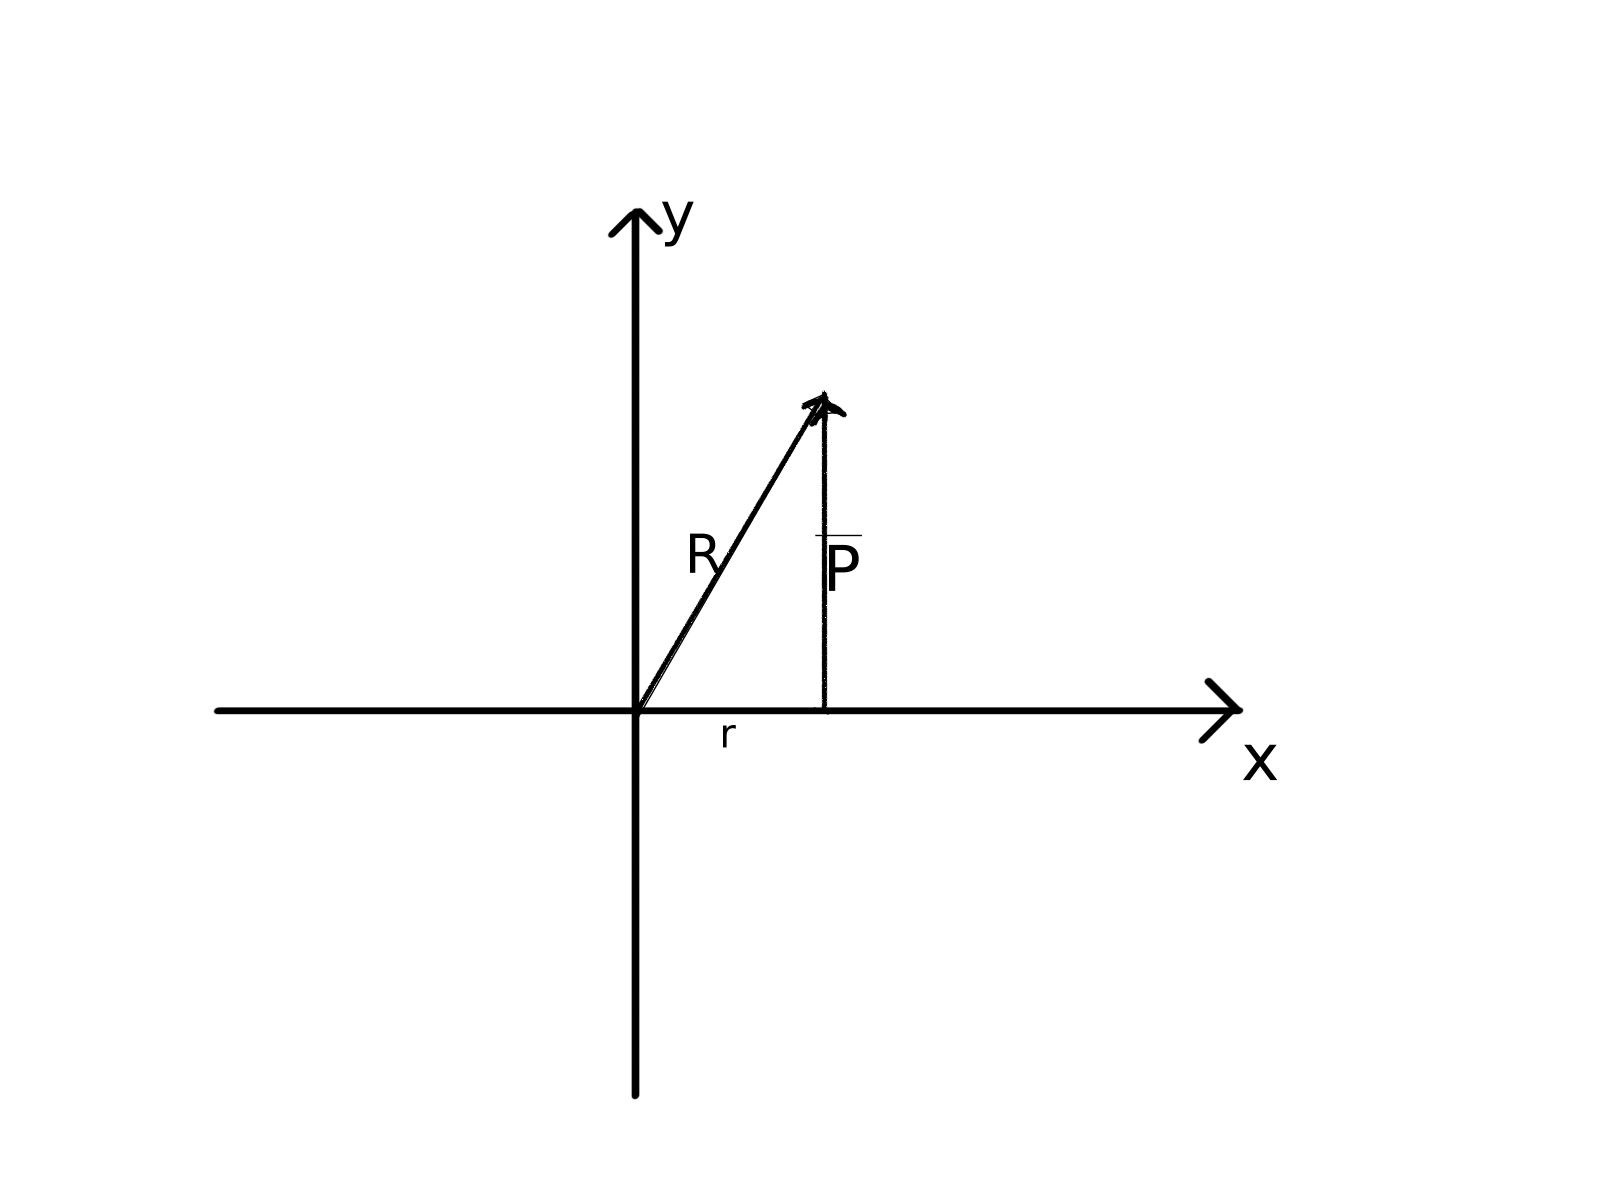
\includegraphics[width=\textwidth]{fig1}
      \captionof{figure}{Vector Diagram}
      \label{vectordiagram}
\end{minipage}

From Figure \ref{vectordiagram}, 

\begin{center}
$ \vec{r} = r.\hat{i} $

$ \vec{R} = R\,(cos \theta \hat{i} + sin \theta \hat{j} ) $

$ \vec{p} = \vec{R}-\vec{r} = (R cos \theta-r) \hat{i} + R sin \theta \hat{j} $


$ \vert \vec{p}\vert = \sqrt{(R cos \theta - r)^{2} + (R sin \theta )^{2} }$

\vspace{0.5\baselineskip}
The Gravitational Potential is given by
\begin{equation}
 d{\Phi}= \frac{GmdM}{\vert \vec{p}\vert} 
\end{equation}


$ \Phi = \int {d{\Phi}} $
  

$ d M = \lambda R d \theta  $
\vspace{0.5\baselineskip}
By substituting Linear Mass Distribution ,
\begin{equation}
\Phi= \frac{GMmR}{2\pi R} \int_{0}^{2\pi} \frac {d \theta } {\vert \vec{p} \vert^\frac{1}{2}}
\end{equation}

\begin{equation}
\label{phi1}
\Phi= \frac{GMm}{2\pi} \int_{0}^{2\pi}  
\frac{d{\theta}}{\sqrt{R^2 - 2 R r \cos \theta + r^2}}
\end{equation}


Substitution of the following parameters in equation \eqref{phi1} gives us \eqref{phi2}

$ d \theta = 2 d \beta $,
$ \theta = \pi - 2 \beta $,
$ \beta = \frac{\pi - \theta}{2} $

\begin{equation}
\label{phi2}
\Phi (\vec{r}) = \frac{GMm}{ \pi} \int_{0}^{\frac{\pi}{2}}  \frac{d \beta }{\sqrt{r^2 + R^2 +2 R r (1 - 2 \sin^2 \beta )}}  
\end{equation}

substituting $ q = r^2 + R^2 + 2 r R$ results in 
\begin{equation}
\Phi (\vec{r}) = \frac{GMm}{ \pi} \frac{1}{\sqrt{q}} \int_{0}^{\frac{ \pi}{2}} \frac{d \beta }{\sqrt{1 - \frac{4 r R}{q} \sin^2 \beta}}   
\end{equation}
 
and then substituting $ k = \sqrt{\frac{4 r R }{q}} $ and $ k^2 = \frac{4 r R}{q} $ results in
\begin{equation}
\label{elliptic}
\Phi (\vec{r}) = \frac{GMm}{ \pi} \frac{1}{\sqrt{q}} \int_{0}^{\frac{ \pi}{2}} \frac{d \beta } {1 - k^2 \sin \beta } 
\end{equation}

We know that the equation \eqref{elliptic} is the Elliptic Integral of the First kind,
\begin{equation}
\frac{d \beta } {1 - k^2 \sin \beta } = K (k) 
\end{equation}
 
Therefore Equation \eqref{elliptic} can be expressed as
\begin{equation}
 \Phi (\vec{r}) = \frac{GMm}{ \pi} \frac{1}{\sqrt{q}} K (k) 
\end{equation}

Force is given by
\begin{equation}
   \vec{F} = - \vec{\nabla} \Phi 
\end{equation}
\end{center}

we know that,
\begin{center}

\begin{equation}
\frac{\partial K (k)}{\partial k } = \frac{E(k)- (1-k^2) K(k)}{k(1- k^2)} 
\end{equation}
\end{center}
where, E(k) is the Eliiptic Integral of Second kind,

\begin{center}

\begin{equation}
 \frac{\partial q}{\partial r} = 2 (r + R)
\end{equation}

\begin{equation}
 \frac{\partial k}{\partial r} = \frac{2R - k^2 (r + R)}{kq} 
\end{equation}

\begin{equation}
\frac{d K(k)}{d k} = \frac{E(k) - (1-k^2) K(k)}{k (1-k^2)} 
\end{equation}

\begin{equation}
\frac{\partial K (r)}{\partial r} = \frac{d K(k)}{dk} \frac{\partial k }{r} 
\end{equation}

\begin{equation}
\frac{\partial \Phi}{\partial r} = - \frac{GMm }{\pi} [ \frac{E(k) - (1-k^2) K(k)}{k (1-k^2)} (\frac{2R - k^2 (r + R)}{kq} \sqrt{q}) - (\frac{\frac{1}{2} \frac{1}{\sqrt{q}}2 (r + R ) K(k)} {q}] 
\end{equation}

\end{center}

Simplifying,

\begin{center}


$ = - \frac{GMm }{\pi} [\frac{\frac{(E(k)- (1 - k^2 )K(k))(2 R - k^2 (r + R)) - (r + R) K(k) k^2 (1 - k^2)}{k^2 (1-k^2)\sqrt{q}}}{q}] $


$ = - \frac{GMm }{\pi} [\frac{2 R E(k) - E (k) k^2 (r+R) - 2 R(1-k^2) K(k)}{k^2 (1 - k^2) q^\frac{3}{2}}] $





\begin{equation}
 = - GMm \frac{1}{\pi k^2 (1 - k ^2)  q^\frac{3}{2}} [2 R E (k) - k^2 r E(k)- k^2 R E(k) - 2 R K(k) + 2 R k^2 K(k)]
\end{equation}

\begin{equation}
 = - GMm \frac{1}{\pi k^2 (1 - k ^2)  q^\frac{3}{2}} [E (k) 2R - k^2 (r + R) - 2 R K(k) (1 - k^2) ] 
\end{equation}
\end{center}
 
substituting,
 \begin{center}
 $ \mu = k^2  $
 \end{center}


The final expression for Gravitational Force is:
\begin{center}

\begin{equation}
 \vec{F}_{r} = - GMm \frac{1}{\pi q^ \frac{3}{2} (1- \mu)} \frac{1}{\mu} (2 R K(\sqrt{\mu}) (1 - \mu))- E (\sqrt{\mu}) (2 R - \mu (r + R))
\end{equation}

\end{center}

\subsection{Data from Histogram}
To calculate force, we require information about the masses of the rings. For that purpose, we extracted data from the Histogram of masses plotted as a function of normalized intensity. In astronomy, we have direct relation between the Luminosity and Masses of a celestial object, i.e. 

\begin{equation}
\frac{L}{L_{\odot}} = (\frac{M}{M_{\odot}})^4 
\end{equation}

So by saving the values of luminosity from the same file, we used in section 2.2.2 , and using the equation (2.24) we get the values of masses for each body.  

\subsection{Function Definition for Data Extraction from Histogram}
\begin{verbatim}

    with open('data.csv', 'w') as fout:

        for x in range(w):
            for y in range (h):

                r= calc_distance(x0,y0,x,y)
                i = calc_gs_intensity( andro[x,y] )
                m= i**0.25 

                print (r,i,m)


                fout.write(str(r) + "," + str(i)+ "," + str(m) + "\n")

\end{verbatim}


\subsection{Function Definition for Calculation of Force}
\begin{verbatim}
def q(r,R) :

    return r*r+R*R+2*r*R

def k(r,R,con) :
    b = float(4*r*R)
    return (b/con)

def f(m,M,R,r,con,ks,g):
    d= 2*R - ks * (r+R)
    E=  ellipe(ks**0.5 )          ##(elliptic function of 2nd kind)
    j= (1-ks)
    G= 2*R* ellipk(ks**0.5)       ## elliptic function of 1st kind
    h= math.pi * (con ** 1.5) *j

    return (((-1*M*ms*g)/ h) * (1/ks)* (G *j -E *d) )

def F(ms,M,R,r):

    # print(r)s
    # print(R)
    con = q(r,R)
    # print (con)
    ks = k(r,R,con)
    # print (ks)
    g = 6.67e-11

    # fa = f(m,M,R,r,con,ks,g)
    # print (fa)


    return f(ms,M,R,r,con,ks,g)

\end{verbatim}

\begin{figure}[h]
\centering
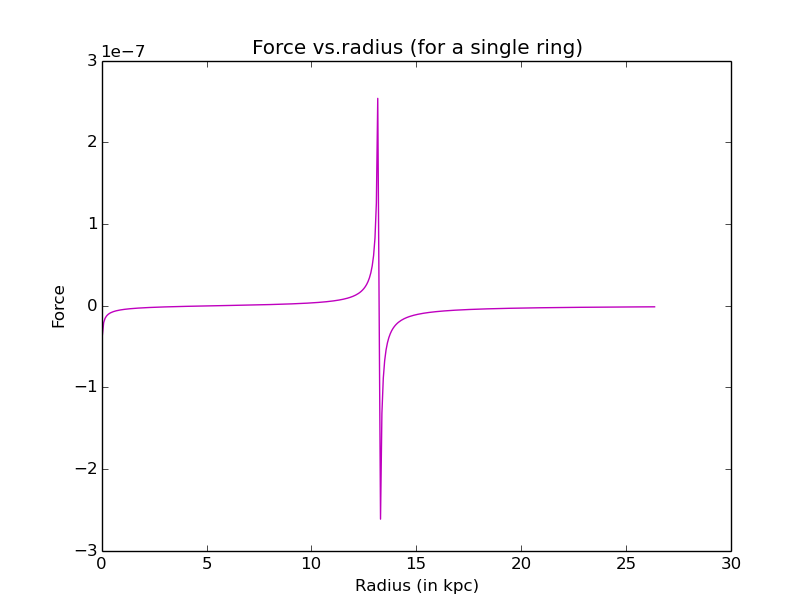
\includegraphics[scale=0.5]{force41R} 
\caption{force on a single ring }
\end{figure}



\section{Calculation for Velocity }

Centripetal force is known to be,

\begin{center}
\begin{equation}
\vec{F_{c} = \frac{m v^2 }{r}}
\end{equation}

\begin{equation}
\vec{F}_{r} = - GMm \frac{1}{\pi q^ \frac{3}{2} (1- \mu)} \frac{1}{\mu} (2 R K(\sqrt{\mu}) (1 - \mu))- E (\sqrt{\mu}) (2 R - \mu (r + R))
\end{equation}

\begin{equation}
v = \sqrt{\frac{GMm \frac{1}{\pi q^ \frac{3}{2} (1- \mu)} \frac{1}{\mu} (2 R K(\sqrt{\mu}) (1 - \mu))- E (\sqrt{\mu}) (2 R - \mu (r + R))}{r}}
\end{equation}

\end{center}

\subsubsection{Function Definition for Velocity}
\begin{verbatim}
 def v(self, rs, v0, m0):

        vs=[]

        self.Mass[0] = m0

        for r in rs:

            T=0

            for i in range(len(self.Rad)):
                R= self.Rad[i]
                M= self.Mass[i]
                if abs(R-r) > 0.5:
                    lF = F(ms,M,R,r)
                    T= T+lF

            v = v0 * (abs(T*r))**0.5
            vs.append(v)

        return vs
\end{verbatim}


\section{Observed Rotation Curve}

The data used in this program is precalculated data of radius in kpc and rotational velocities in $kms^{-1}$ for Andromeda Galaxy.\cite{observed} 
\begin{verbatim}

x= []
y= []

with open ('rd.txt','r') as f:
    for row in f:

        x.append((row)) #appends the data in empty list for distances



with open ('vrot.txt', 'r') as f1:
    for row1 in f1:

        y.append((row1)) #appends the data in empty list for rotational velocities.


pylab.ylim([0,400])
pylab.xlim([0,35])
plt.plot(x,y)
plt.scatter(x,y)


\end{verbatim}

\section{Optimization of Velocity and Mass}
The velocities and masses according to the calculated data were not able to regenerate the rotation curve as required, so curve fitting was reqquired. In the program below, we optimize the calculated curve according to the observed and get the values of parameters as $v_{0}$ and $m_{0}$
\begin{verbatim}
a,b = scipy.optimize.curve_fit(fit.v, R, V)
    print (a)
    print b


    v0 = a[0]
    m0 = a[1]
    v = fit.v(R,v0,m0)   #for black hole mass
    pmv = plt.scatter(R,v, color= 'g',label ='m0 & v0')
    plt.plot(R,v)


    vo = fit.v(R,v0,m0_o)  #for very small mass .. i.e the first entry in the list.
    pv = plt.scatter(R,vo , color='y', label = 'v0')
    plt.plot(R,vo)
\end{verbatim}




